\documentclass[border=1cm]{standalone}
\usepackage{tikz}
\usetikzlibrary{math}

\newcommand\Square[2]{
  \fill #1 rectangle ++(#2,#2);
}

\begin{document}
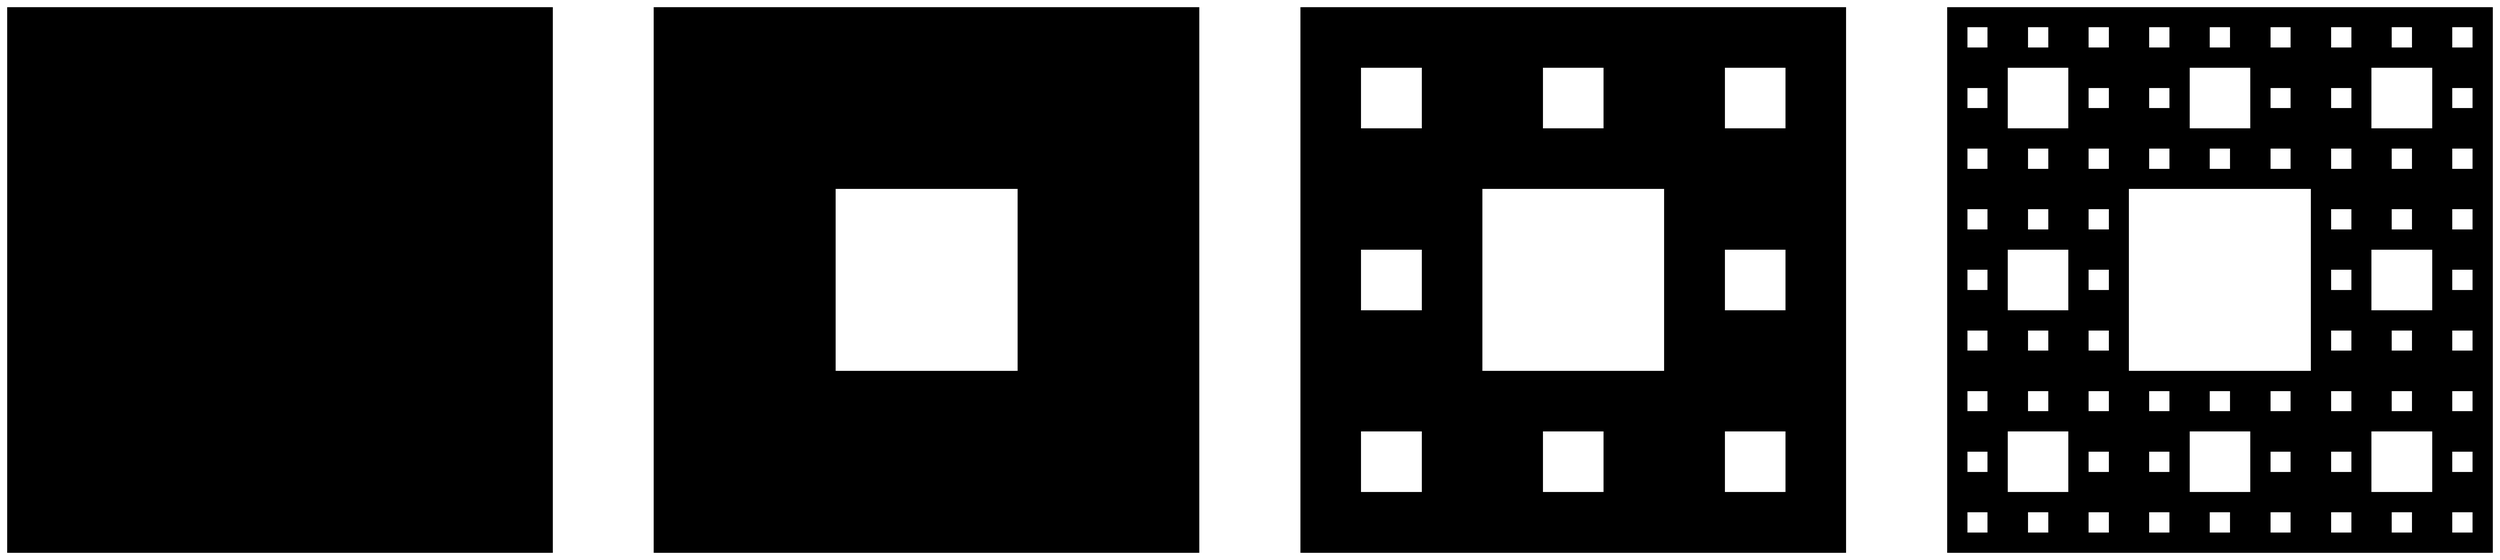
\begin{tikzpicture}
  \tikzmath{
    function carpet(\x, \y, \s, \d) {
      if (\d == 0) then {
        { \Square{(\x,\y)}{\s}; };
      } else {
        \u = \s / 3;
        for \i in {0,1,2}{
          for \j in {0,1,2}{
            if !(\i==1 && \j==1) then {
              carpet(\x + \i*\u, \y + \j*\u, \u, \d-1);
            };
          };
        };
      };
    };
    \S = 27;
    for \d in {0,1,2,3}{
      \px = (\S + 5) * \d;
      \py = 0;
      carpet(\px, \py, \S, \d);
    };
  }
\end{tikzpicture}
\end{document}
